\documentclass[a4paper]{article}
    \usepackage{minted}
    \usepackage{xcolor}
    \usepackage[colorlinks,linkcolor=black]{hyperref}
    \usepackage[margin=1in]{geometry}
    \usepackage{caption}
    \usepackage{graphicx}
    \usepackage{subfigure}
    \usepackage{float}
    \usepackage{fontspec}
    \setmainfont{Times New Roman}
    \setmonofont{Consolas}
    \definecolor{bg}{rgb}{0.9,0.9,0.9}
    \usemintedstyle{manni}
    \setminted{
    linenos,
    autogobble,
    breaklines,
    breakautoindent,
    bgcolor=bg,
    numberblanklines=false,
    }

\begin{document}
    \tableofcontents
    \newpage
    \section{Preparations}
        \subsection{Analysis}
As required, the final project is nearly a complete website, which is composed of pages of search, paper, author,
conference and affiliation. To implement these pages, both back-end and front-end works are needed. 

As for the provided optional features, after some careful consideration, I don't think all of them are appropriate.
For example, the mentorship graph seems good but actually, it contains too much information and looks ugly and untidy
(as far as that of Acemap is concerned).

Therefore, I decide not to fully follow the given suggestions but to implement something more practical and graceful.  
        \subsection{Overall Design}
Before I begin to dive into coding, I first design the overall appearances and functions of the website. 
My design manuscript looks like these, quite rough but useful:
\begin{figure}[H]
\begin{minipage}[t]{0.5\linewidth}  
\centering  
\includegraphics[width=2.2in]{img/manuscript1.jpg}  
\caption{Manuscript 1}  
\label{fig:side:a}  
\end{minipage}%  
\begin{minipage}[t]{0.5\linewidth}  
\centering  
\includegraphics[width=2.2in]{img/manuscript2.jpg}  
\caption{Manuscript 2}  
\label{fig:side:b}  
\end{minipage}  
\end{figure}
        \subsection{Overall Structure}
As I work with CodeIgniter, the overall structure of the website is: first, the router handles the URL and calls
the Controller; then the Controller gets necessary data from the Model and passes them to the View; and finally,
the View renders the HTML page. 

For some dynamic functions like pagination, the browser uses JavaScript to send query to the server and then update 
the current page.
    \newpage
    \section{Back-end}
The back-end can be divided into mainly two parts: Page and API. The former handles usual queries and 
renders HTML pages while the latter is designed to provide raw data encoded in JSON for the front-end.
        \subsection{Page}
As has been illustrated in the previous reports, a Contoller named \mintinline{php}{Page} is implemented, which contains member
functions like:
\begin{minted}{php}
<?php
public function index()
public function result($query=NULL)
public function author($authorID=NULL)
public function paper($paperID=NULL)
public function conference($conferenceID=NULL)
public function affiliation($affiliationID=NULL)
public function about()
?>
\end{minted}
These functions handle different pages like home, search result and author. To make this report compact, I only
illustrate the first two functions.

In the home page, the user can enter the query string and also select the types of search. So \mintinline{php}{index()}
handles the input, encodes the search type into a string containing 0s and 1s and redirects the user to the search result:
\begin{minted}{php}
<?php
    public function index()
    {
        $this->load->helper('form');
        $this->load->library('form_validation');
        $this->form_validation->set_rules('queryString', 'Query String', 'required');
        $this->form_validation->set_rules('type[]','Search Type','required');
        if ($this->form_validation->run() === FALSE){
            $this->load->view('templates/home.php');
        }
        else{
            $queryString=$this->input->post("queryString");
            $type="";
            $allTypes=array("author","paper","conference","affiliation");
            for($i=0;$i!=4;$i++){
                if(in_array($allTypes[$i],$this->input->post("type[]"))){
                    $type.="1";
                }
                else
                    $type.="0";
            }
            redirect("/result/$queryString?type=$type");
        }
    }
?>  
\end{minted}
Then, it's time for \mintinline{php}{result()}. According to the search type( something like 0110), it
provides different search results. And if the search type is not set correctly, it will handle it as default.
The code looks like these:
\begin{minted}{php}
<?php
    public function result($query=NULL)
    {
        if(!$query){
            $data["title"]="Error";
            $data["errorMsg"]="Invalid Query!";
            $this->load->view("templates/header.php",$data);
            $this->load->view("templates/error.php",$data);
            $this->load->view("templates/footer.php");
        }else{
            $queryString=str_replace("%20", " ", $query);
            $type=$this->input->get_post("type");
            if(strlen($type)!=4 or $type=="0000")
                $type="1111";
            $data["title"]="Search result of ".ucwords($queryString);
            $data["resultNum"]=0;
            $data["script"]="
            var query='$query';";
            if($type[0]){
                $data["authorNum"]=$this
                    ->Search_result_model->get_author_number($queryString);
                $data["authorResult"]=$this
                    ->Search_result_model->get_author_result($queryString);
                $data["resultNum"]+=$data["authorNum"];
                $pageSize=10;
                $maxPage=(int)(($data["authorNum"]-1)/$pageSize)+1;
                $data["authorMaxPage"]=$maxPage;
                $data["script"].="
                var authorCurrentPage=1;
                var authorPageSize=$pageSize;
                var authorMaxPage=$maxPage;
                var authorApiUrl='/api/search/author';
                $(function(){checkButtonStatus('author');})
                ";
            }
            if($type[1]){}  //ommited
            if($type[2]){}  //ommited
            if($type[3]){}  //ommited
            $this->load->view("templates/header.php",$data);
            $this->load->view("templates/result.php",$data);
            $this->load->view("templates/footer.php");
        }   
    }
?>
\end{minted}
You might have noticed that in the code, the function calls other functions in \mintinline{php}{Search_result_model}.
You can know what these functions do by their names, such as \mintinline{php}{get_author_number} or view their code
in the attached files. So for the sake of conciseness, I just skip them and other things about Models here.

As for the other functions, they work in a similar way: first get query, then call some functions in some Model
to get necessary data, and eventually pass the data to some Views.
        \subsection{API}
Considering the functions of the website, the API mainly has three functions: \mintinline{php}{search()}, 
\mintinline{php}{get_papers()} and \mintinline{php}{graph()}. Also, I only illustrate the first two of them here.
            \subsubsection{Search}
As has been mentioned above, there are four types of search. To handle different search types, using switch and case
is an common way, but using the feature of PHP, variable functions, things can be easier and more graceful. 

This feature enables us to call a function by the value of a variable and thus saves a lot of code. So the function looks
like this:
\begin{minted}{php}
<?php
    public function search($type=NULL,$query=NULL,$page=1,$pageSize=10)
    {
        $json=array();
        $data=array();
        if(!$query or !$type){
            $json["success"]=0;
            $json["reason"]="The query or type is NULL.";
        }else if(in_array($type, array("author","paper","conference","affiliation"))==false){
            $json["success"]=0;
            $json["reason"]="Invalid search type!";
        }else{
            $get_result_number="get_".$type."_number";  //Attention here!
            $resultNum=$this->Search_result_model->$get_result_number($query);
            if($resultNum==0){
                $json["success"]=0;
                $json["reason"]="No result found.";
            }else{
                $maxPage=(int)(($resultNum-1)/$pageSize) + 1;
                if($page>$maxPage){
                    $json["success"]=0;
                    $json["reason"]="Out of page limit.";
                    $json["resultNum"]=$resultNum;
                    $json["pageSize"]=$pageSize;
                    $json["maxPage"]=$maxPage;
                    $json["page"]=$page;
                    $json["itemNum"]=0;
                }else{
                    $json["success"]=1;
                    $json["resultNum"]=$resultNum;
                    $json["pageSize"]=$pageSize;
                    $json["maxPage"]=$maxPage;
                    $json["page"]=$page;
                    $begin=$pageSize*($page-1);
                    $get_search_result="get_".$type."_result";  //Attention!
                    $json["searchResult"] = 
                        $this->Search_result_model
                        ->$get_search_result($query,$begin,$pageSize);
                    $json["itemNum"]=count($json["searchResult"]);
                }
            }
        }
        $data["json"]=$json;
        $this->load->view("templates/json.php",$data);
    }
?>    
\end{minted}
As you can see, according to the search type, \mintinline{php}{$get_result_number} changes and thus the function
to call changes. So this feature is really useful and powerful.
            \subsubsection{Get Papers}
There're many pages that need to get the data of papers, such as the page of paper and the page of author. So to
integrate all the queries for papers, a variable \mintinline{php}{$type} is needed. Then according to the value
of it, different functions in different models are called using the feature mentioned above.
\begin{minted}{php}
<?php
    public function get_papers($type=NULL,$ID=NULL,$page=1,$pageSize=10)
    {
        $json=array();
        $data=array();
        if(!$ID or !$type){
            $json["success"]=0;
            $json["reason"]="Please specify the ID.";
        }
        switch($type){
            case "author":
                $paperNum=$this->Author_info_model->get_paper_number($ID)["all"];
                $model="Author_info_model";
                $function="get_papers";
                break;
            case "citing-this":
                //omitted
                break;
            case "cited-by-this":
                //omitted
                break;
            case "conference":
                //omitted
                break;
            case "affiliation":
                //omitted
                break;
            default:
                $json["success"]=0;
                $json["reason"]="Invalid type!";
                $data["json"]=$json;
                $this->load->view("templates/json.php",$data);
                return;         
        }   
        if($paperNum==0){
            $json["success"]=0;
            $json["reason"]="No paper found!";
        }else{
            $maxPage=(int)(($paperNum-1)/$pageSize)+1;
            if($page>$maxPage){
                $json["success"]=0;
                $json["paperNum"]=(int)$paperNum;
                $json["pageSize"]=(int)$pageSize;
                $json["maxPage"]=(int)$maxPage;
                $json["page"]=(int)$page;
                $json["reason"]="Out of page limit!";
            }else{
                $json["success"]=1;
                $json["paperNum"]=(int)$paperNum;
                $json["pageSize"]=(int)$pageSize;
                $json["maxPage"]=(int)$maxPage;
                $json["page"]=(int)$page;
                $begin=$pageSize*($page-1);
                $json["papers"]=    //attention here
                    $this->$model->$function($ID,$begin,$pageSize);
                $json["itemNum"]=count($json["papers"]);
            }
        }
        $data["json"]=$json;
        $this->load->view("templates/json.php",$data);
    }
?>  
\end{minted}
Though the switch and case structure can't be avoided in the code above, using the feature of PHP enables the common part
of different branches to be reused. 
    \newpage
    \section{Front-end}
        \subsection{Design}
As I am not skillful in front-end, my aim is not to make the website fancy but neat and clear. 

To achieve this, it's important to keep all the pages uniform. Therefore, I set a fixed 
font(Quicksand) and font size as default for most of the elements in pages.
\begin{minted}{CSS}
body{
    background-image: url(/static/img/bg.png);
    font-size: 25px;
    font-family: 'Quicksand', sans-serif;
    width:100%;
    height:100%;
    min-width: 1300px;
    margin:0;
}
\end{minted} 
Also, I choose \#1abc9c(light green) as the theme color for the website, which is applied to all active elements
such as clickable buttons and links. 
\begin{minted}{CSS}
a {
    text-decoration: none;
    color:#1abc9c;
}
\end{minted}
Then, as in my design, results are displayed in blocks, it's helpful to implement a result container template.
\begin{minted}{CSS}
.resultContainer{
    background-color: #f5f6fa;
    border-style: none;
    padding: 20px;
    margin-bottom:60px;
}

.titleOfContainer{
    width: 100%;
    height:40px;
    background-color: #1abc9c;
    padding-top: 5px;
}

.titleOfContainer a{
    margin-left: 20px;
    color:white;  
}  
\end{minted}
Then when I need a result container, things are quite easy. For example, a snippet of author page looks like this:
\begin{minted}{html}
<div>
    <div class="titleOfContainer">
        <a href="#papers" name="papers">Paper(s)</a>
    </div>
    <div class="resultContainer">
        <div class="overallResult">
            <p>100 papers are found.</p>
        </div>              
        <table id="authorPapersTable" class="resultTable">
            //omitted 
        </table>
            <div class="pagination">
                <button type="button" class="resultPrev" disabled="disabled">Previous</button>
                <span class="pageInfo">
                    //omitted
                </span>
                <button type="button" class="resultNext">Next</button>
            </div>
    </div>
</div>
\end{minted}
And as designed, most pages like author pages are divided into left and right columns. Therefore, in such
pages, the layout is in this way:
\begin{minted}{html}
<div class="mainContainer">
    <div class="leftContainer">
    </div>
    <div class="rightContainer">
    </div>
</idv>
\end{minted}
\begin{minted}{CSS}
.leftContainer{
    width:23%;
    float:left;
}

.rightContainer{
    margin-left: 2%;
    width:75%;
    float:left;
}
\end{minted} 
With all these, the basis of front-end are established.
        \subsection{Graph}
In lab 4, the author relation graph is implemented. And beyond that, I implement quite a few other graphs:

In author page's left part, I add a tag cloud graph, which displays the most frequently occurred words in the title of
the author's papers to give the user a clear impression about the author's research field.

In author page's right part, I add a line graph, which displays how many papers the author publishs yearly and 
shows the trend of his/her academic activity.

In paper page's right part, there's a line graph showing its yearly citations, from which we can gain a insight
into the popularity of its research field.

In conference and affiliation page's right part, a line graph of its yearly number of papers may reveal its
academic influence.

This time, source code files are attached,  so I don't paste code of these graph here. And if you are interested, 
you can find their code in \mintinline{html}{codeigniter/static/js}.
    \newpage
    \section{Speed}
        \subsection{Database Optimization}
Due to the size of the database and sometimes unavoidable queries like \mintinline{sql}{like '%str%'},
it takes quite a few time to load a page. To speed up, the database needs to be optimized.

The most direct way is to add indexes to tables, which is involved in lab 1 and I just skip here. Besides,
changing the structure of the database also works.

For example, as we frequently query for the citations of a paper, it's a good idea to add another column in the
papers table, citations, and then use Python to fill the column. Also, for author relationship, it's better
to create a new table, author\_relation, to store their relations.

In this way, when loading a page, the queries can be much faster.
        \subsection{AJAX}
As in some pages, there are a huge amount of data. For instance, in author page, the data for graphs are enormous.
Therefore, using AJAX to load these data can speed up the loading. The code may look like this:
\begin{minted}{javascript}
d3.json(jsonSource, function(error, data) {
    //do something
});

$(function(){
    //do somethings             
});
\end{minted} 
        \subsection{CDN}
When linking to remote resources like jQuery and D3.js, it’s a good idea to load them from CDNs rather than 
from their original sources. 

In particular, as I use Google Font in the website, it’s extremely slow to load the font from Google and 
sometimes it even fails. So, I use a mirror of Google Font in China. After that, it only takes nearly 10\% 
of time to load the font.
    \newpage
    \section{Security}
Apart from functions and speed, security is vital for a website. Fortunately, as I use CodeIgniter, many things
have been handled automatically. But besides, there're still something to do:
        \subsection{Query Filter}
Before executing a query, it's always necessary to filter it to prevent potential dangers. In CodeIgniter, things
might look like this:
\begin{minted}{php}
<?php
    $sql = "INSERT INTO table (title) VALUES(".$this->db->escape($input).")";
?>
\end{minted}
        \subsection{Database User}
Though it's convenient to connect to the database with "root" user, it's better to use a low-privileged user.
So first, in MySQL, create a low-privileged user:
\begin{minted}{bash}
    grant SELECT on `database`.* to 'username'@'localhost' identified by 'password'; 
\end{minted}
Then in CodeIgniter's config file, use this user to connect to the database.
    \newpage
    \section{Final Result}
Some screenshots of the website:
            \begin{figure}[H]
            \centering
            
\includegraphics[width=.8\textwidth]{img/img6.jpg}
            \caption{Home}
            \end{figure}
                        \begin{figure}[H]
            \centering
            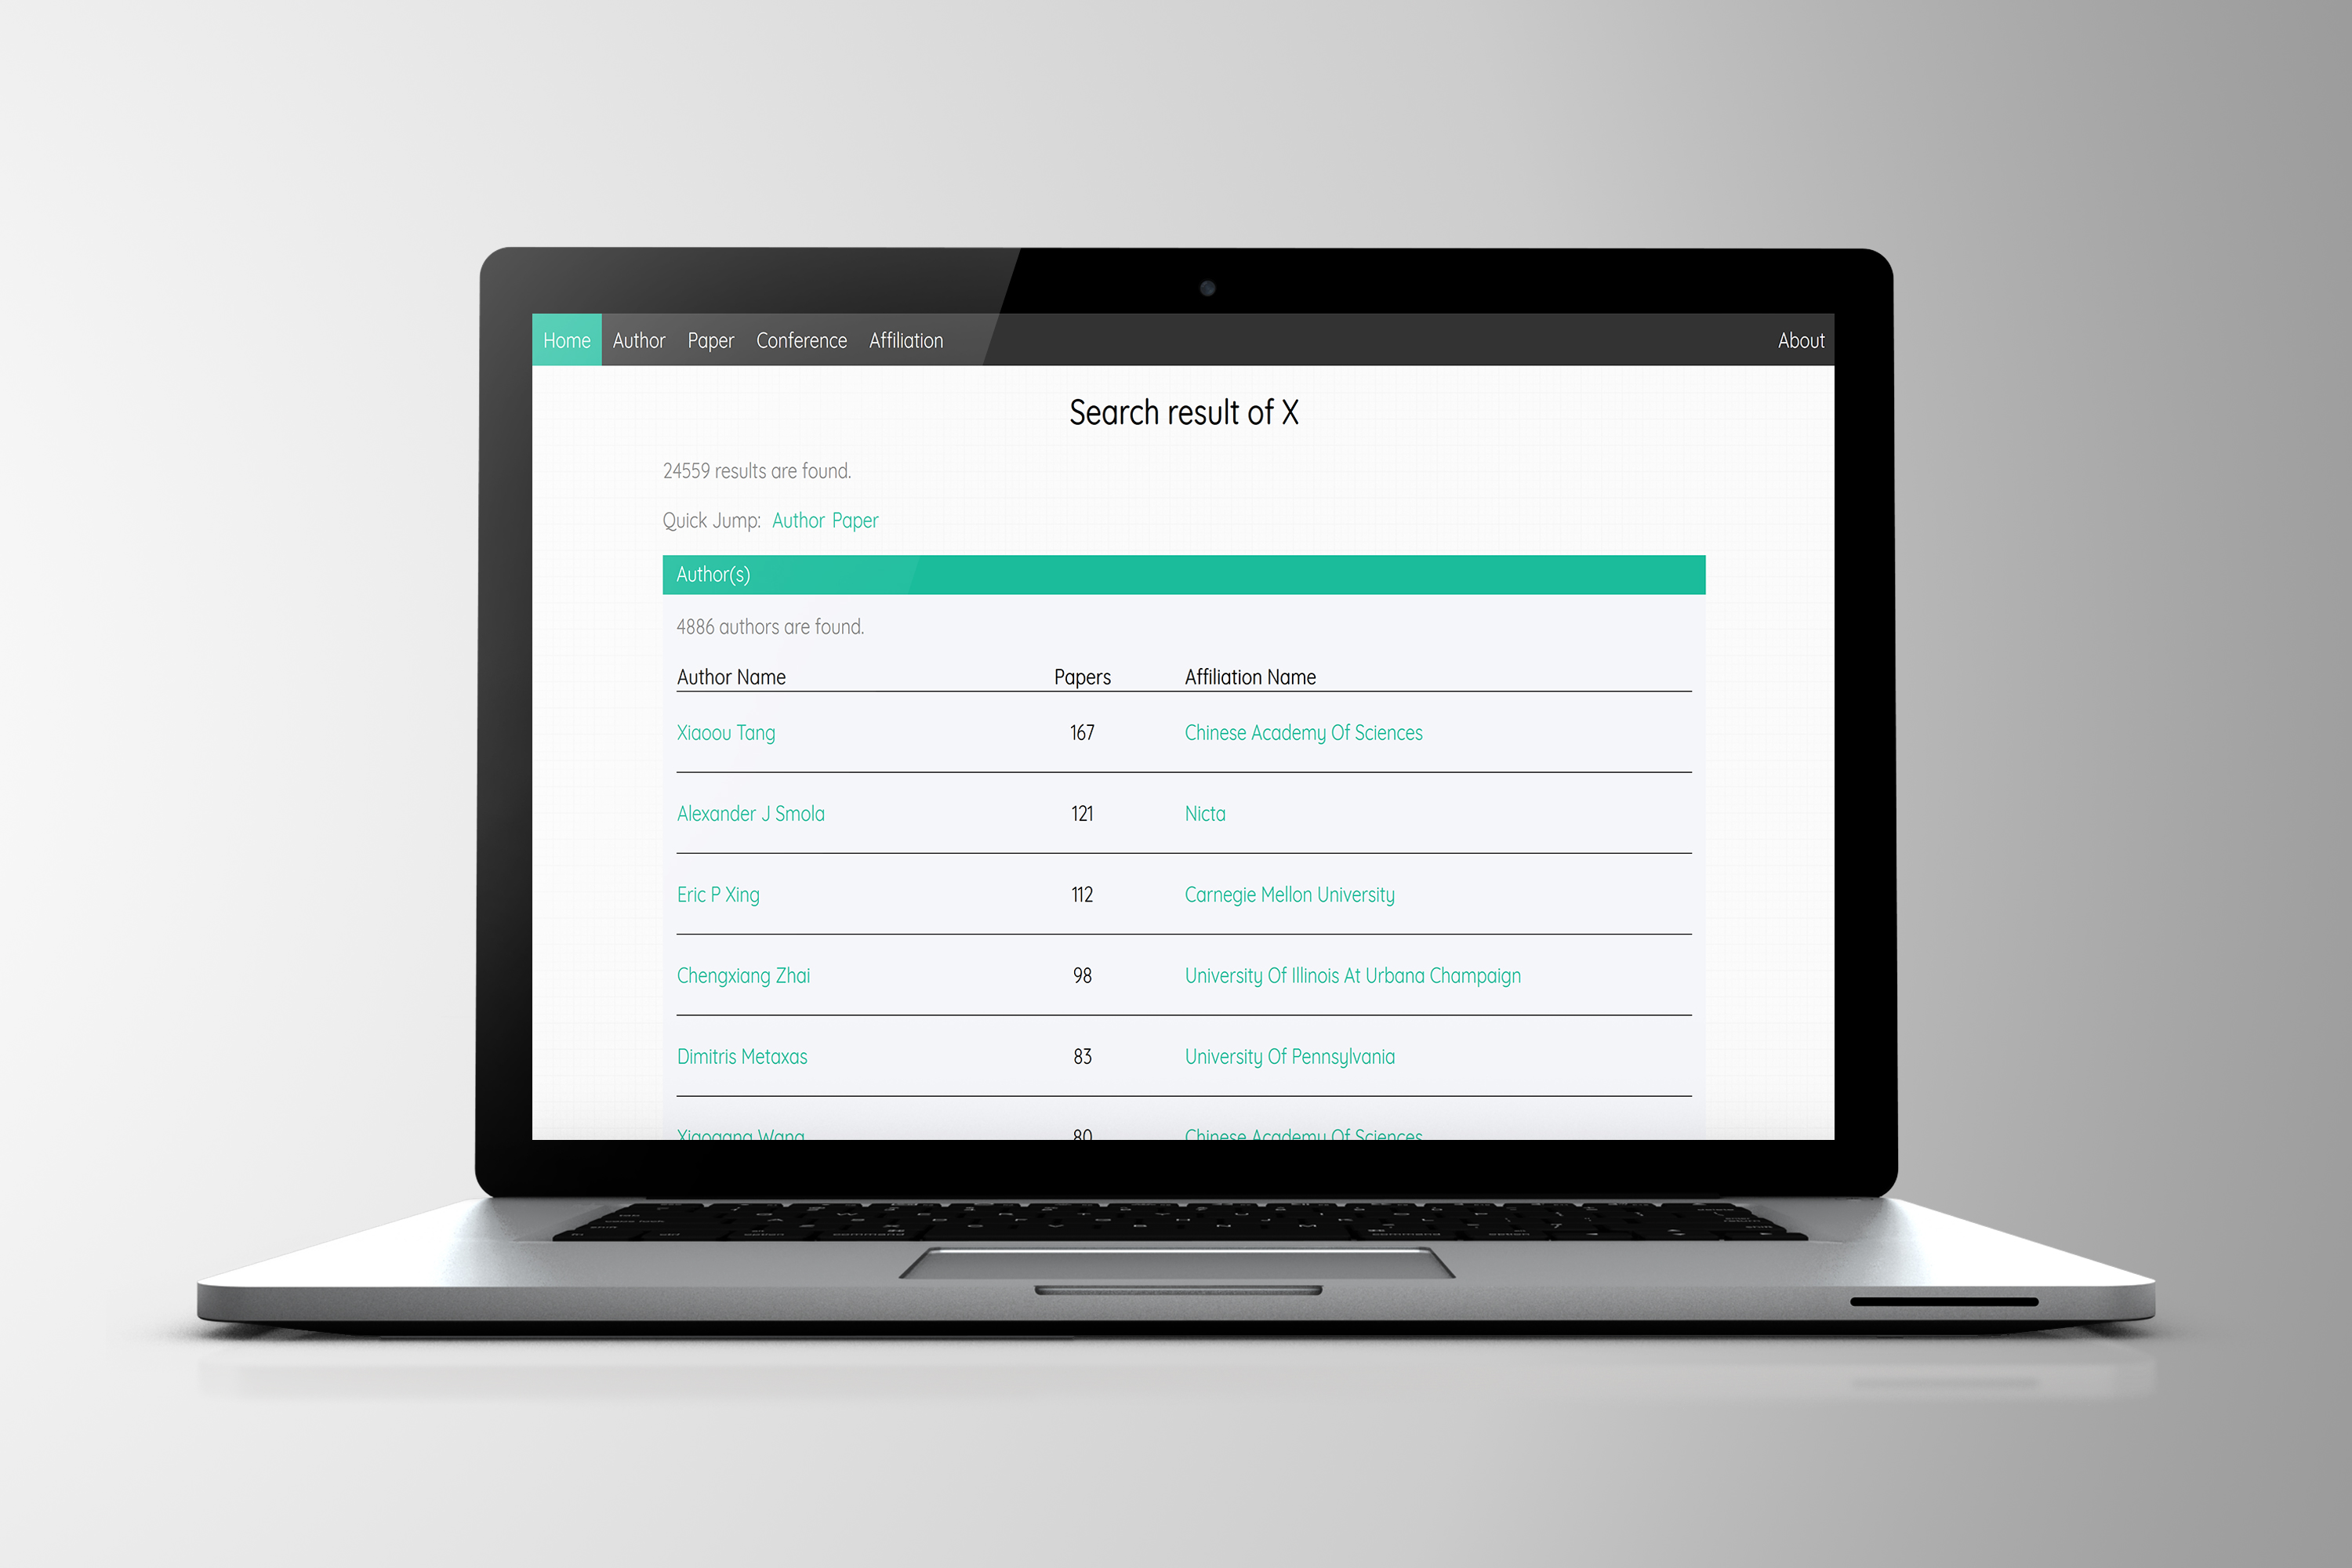
\includegraphics[width=.8\textwidth]{img/img7.jpg}
            \caption{Search Result}
            \end{figure}
                        \begin{figure}[H]
            \centering
            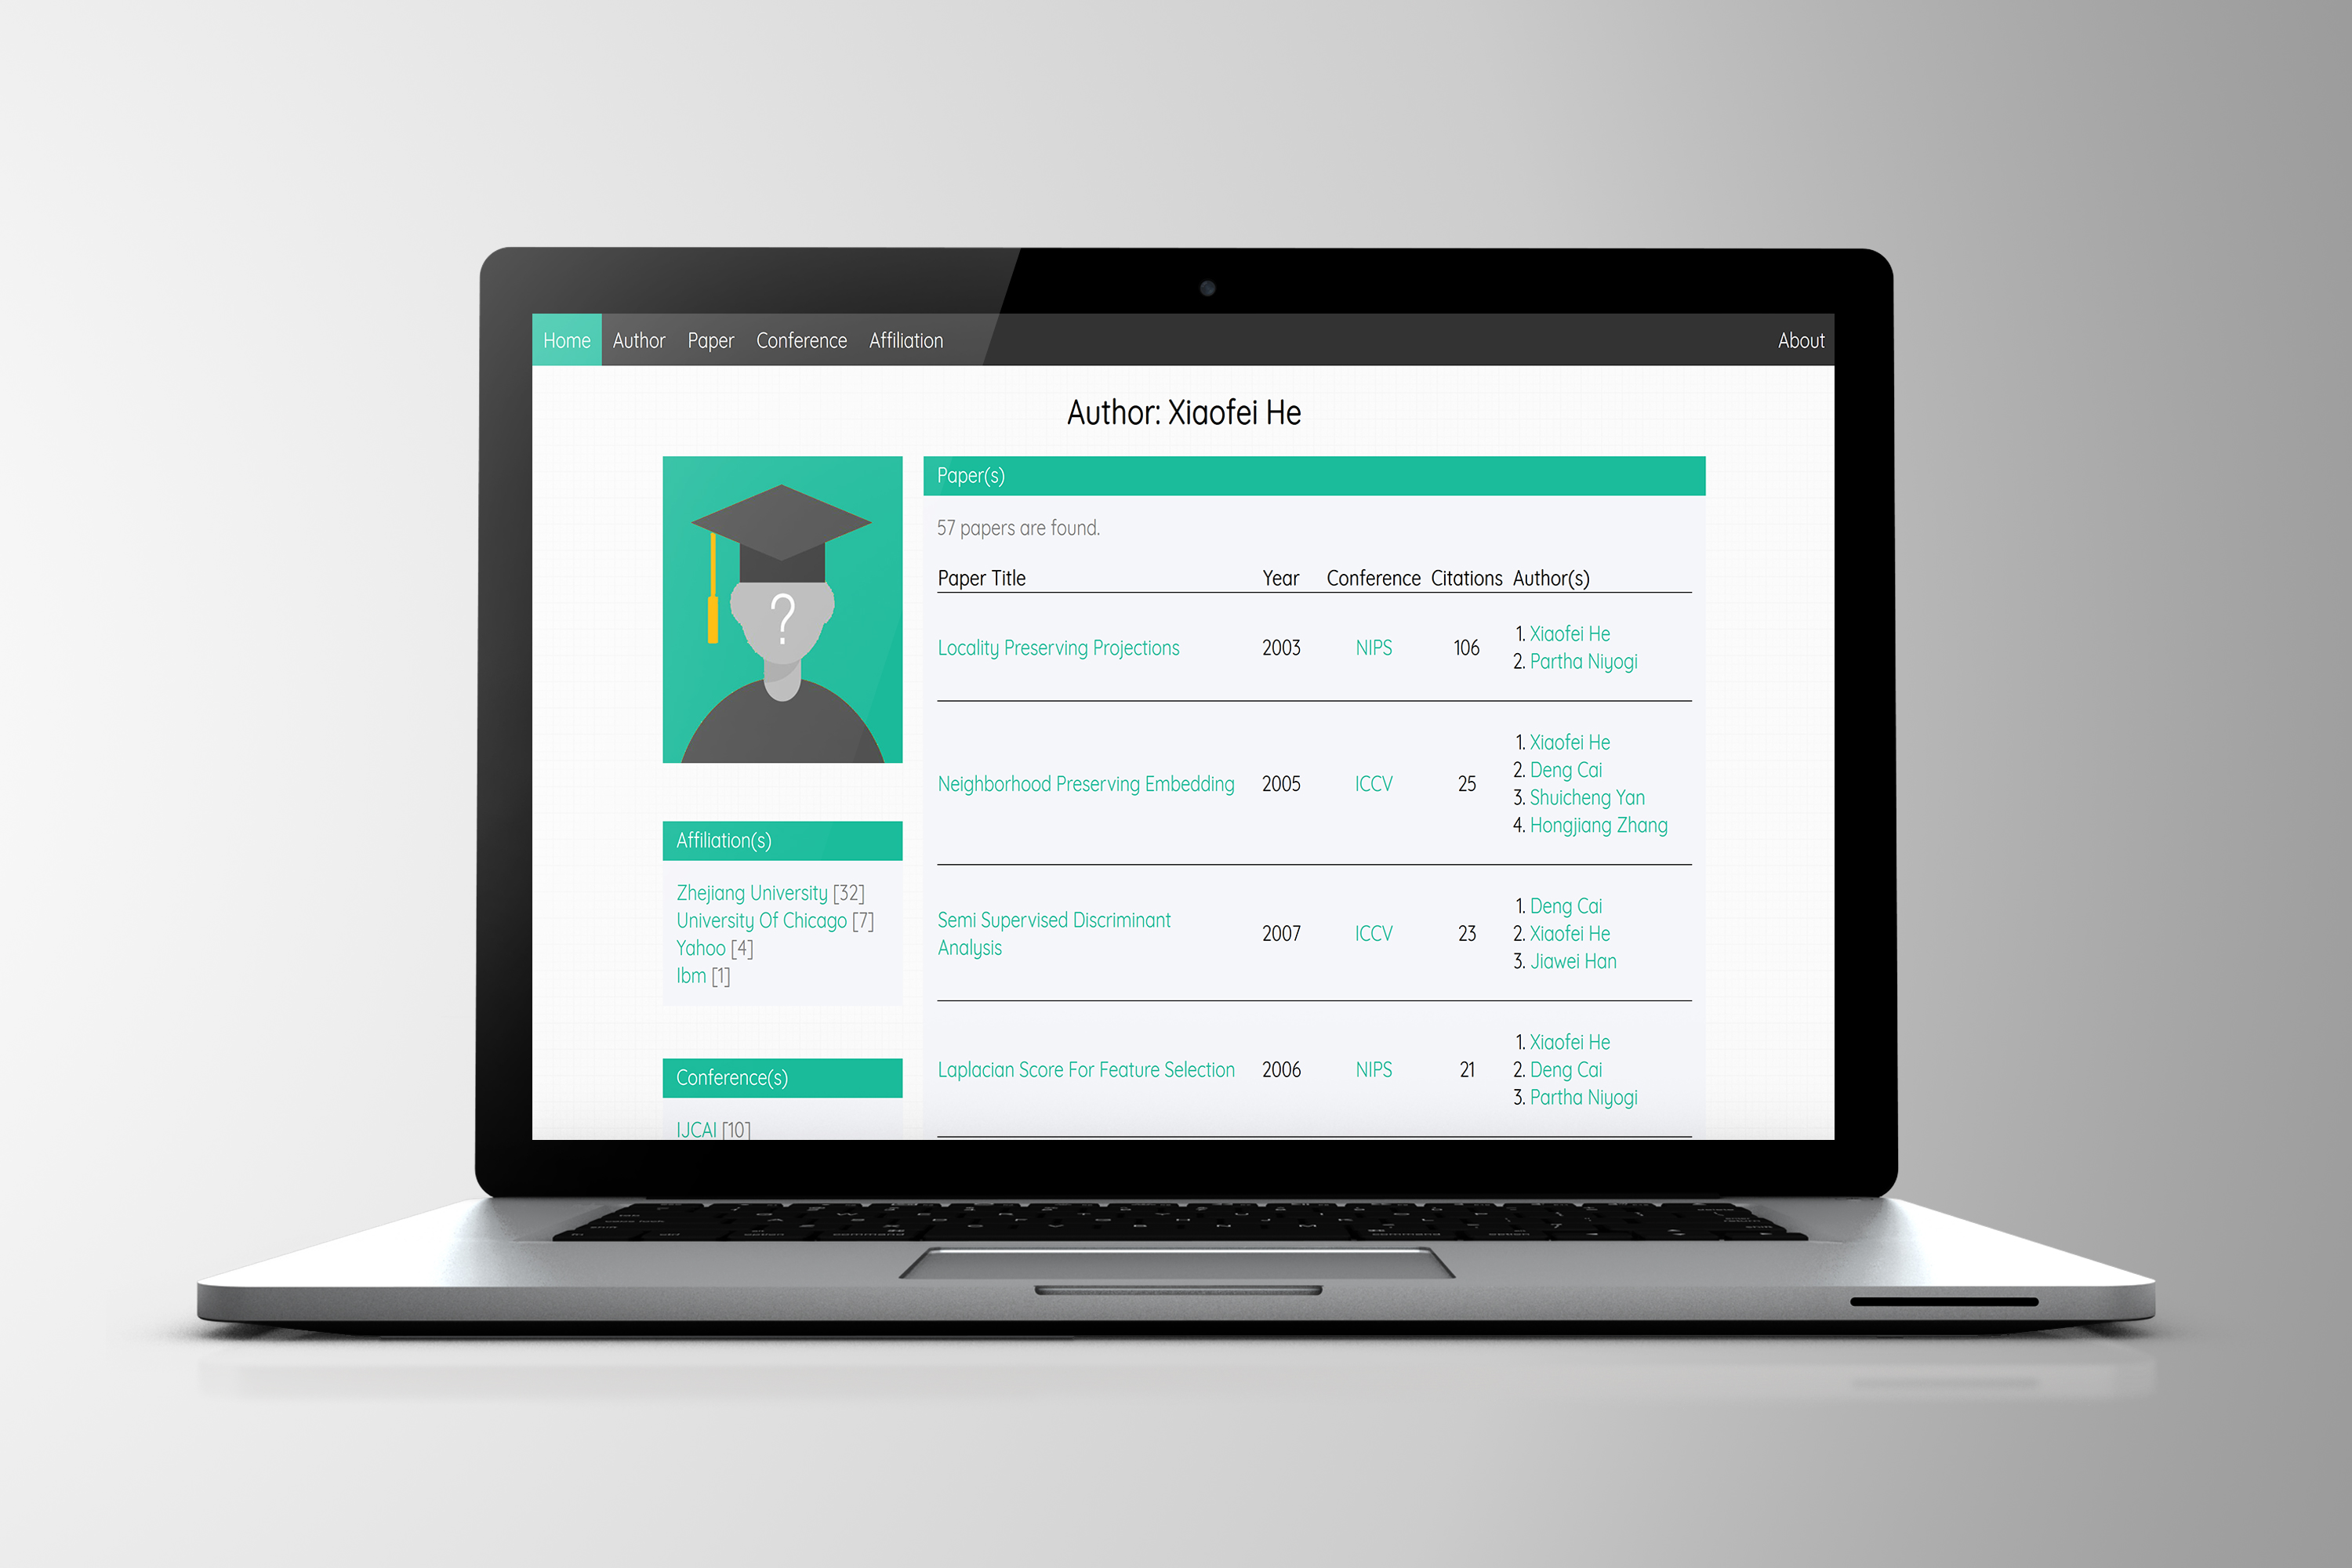
\includegraphics[width=.8\textwidth]{img/img2.jpg}
            \caption{Author}
            \end{figure}
                        \begin{figure}[H]
            \centering
            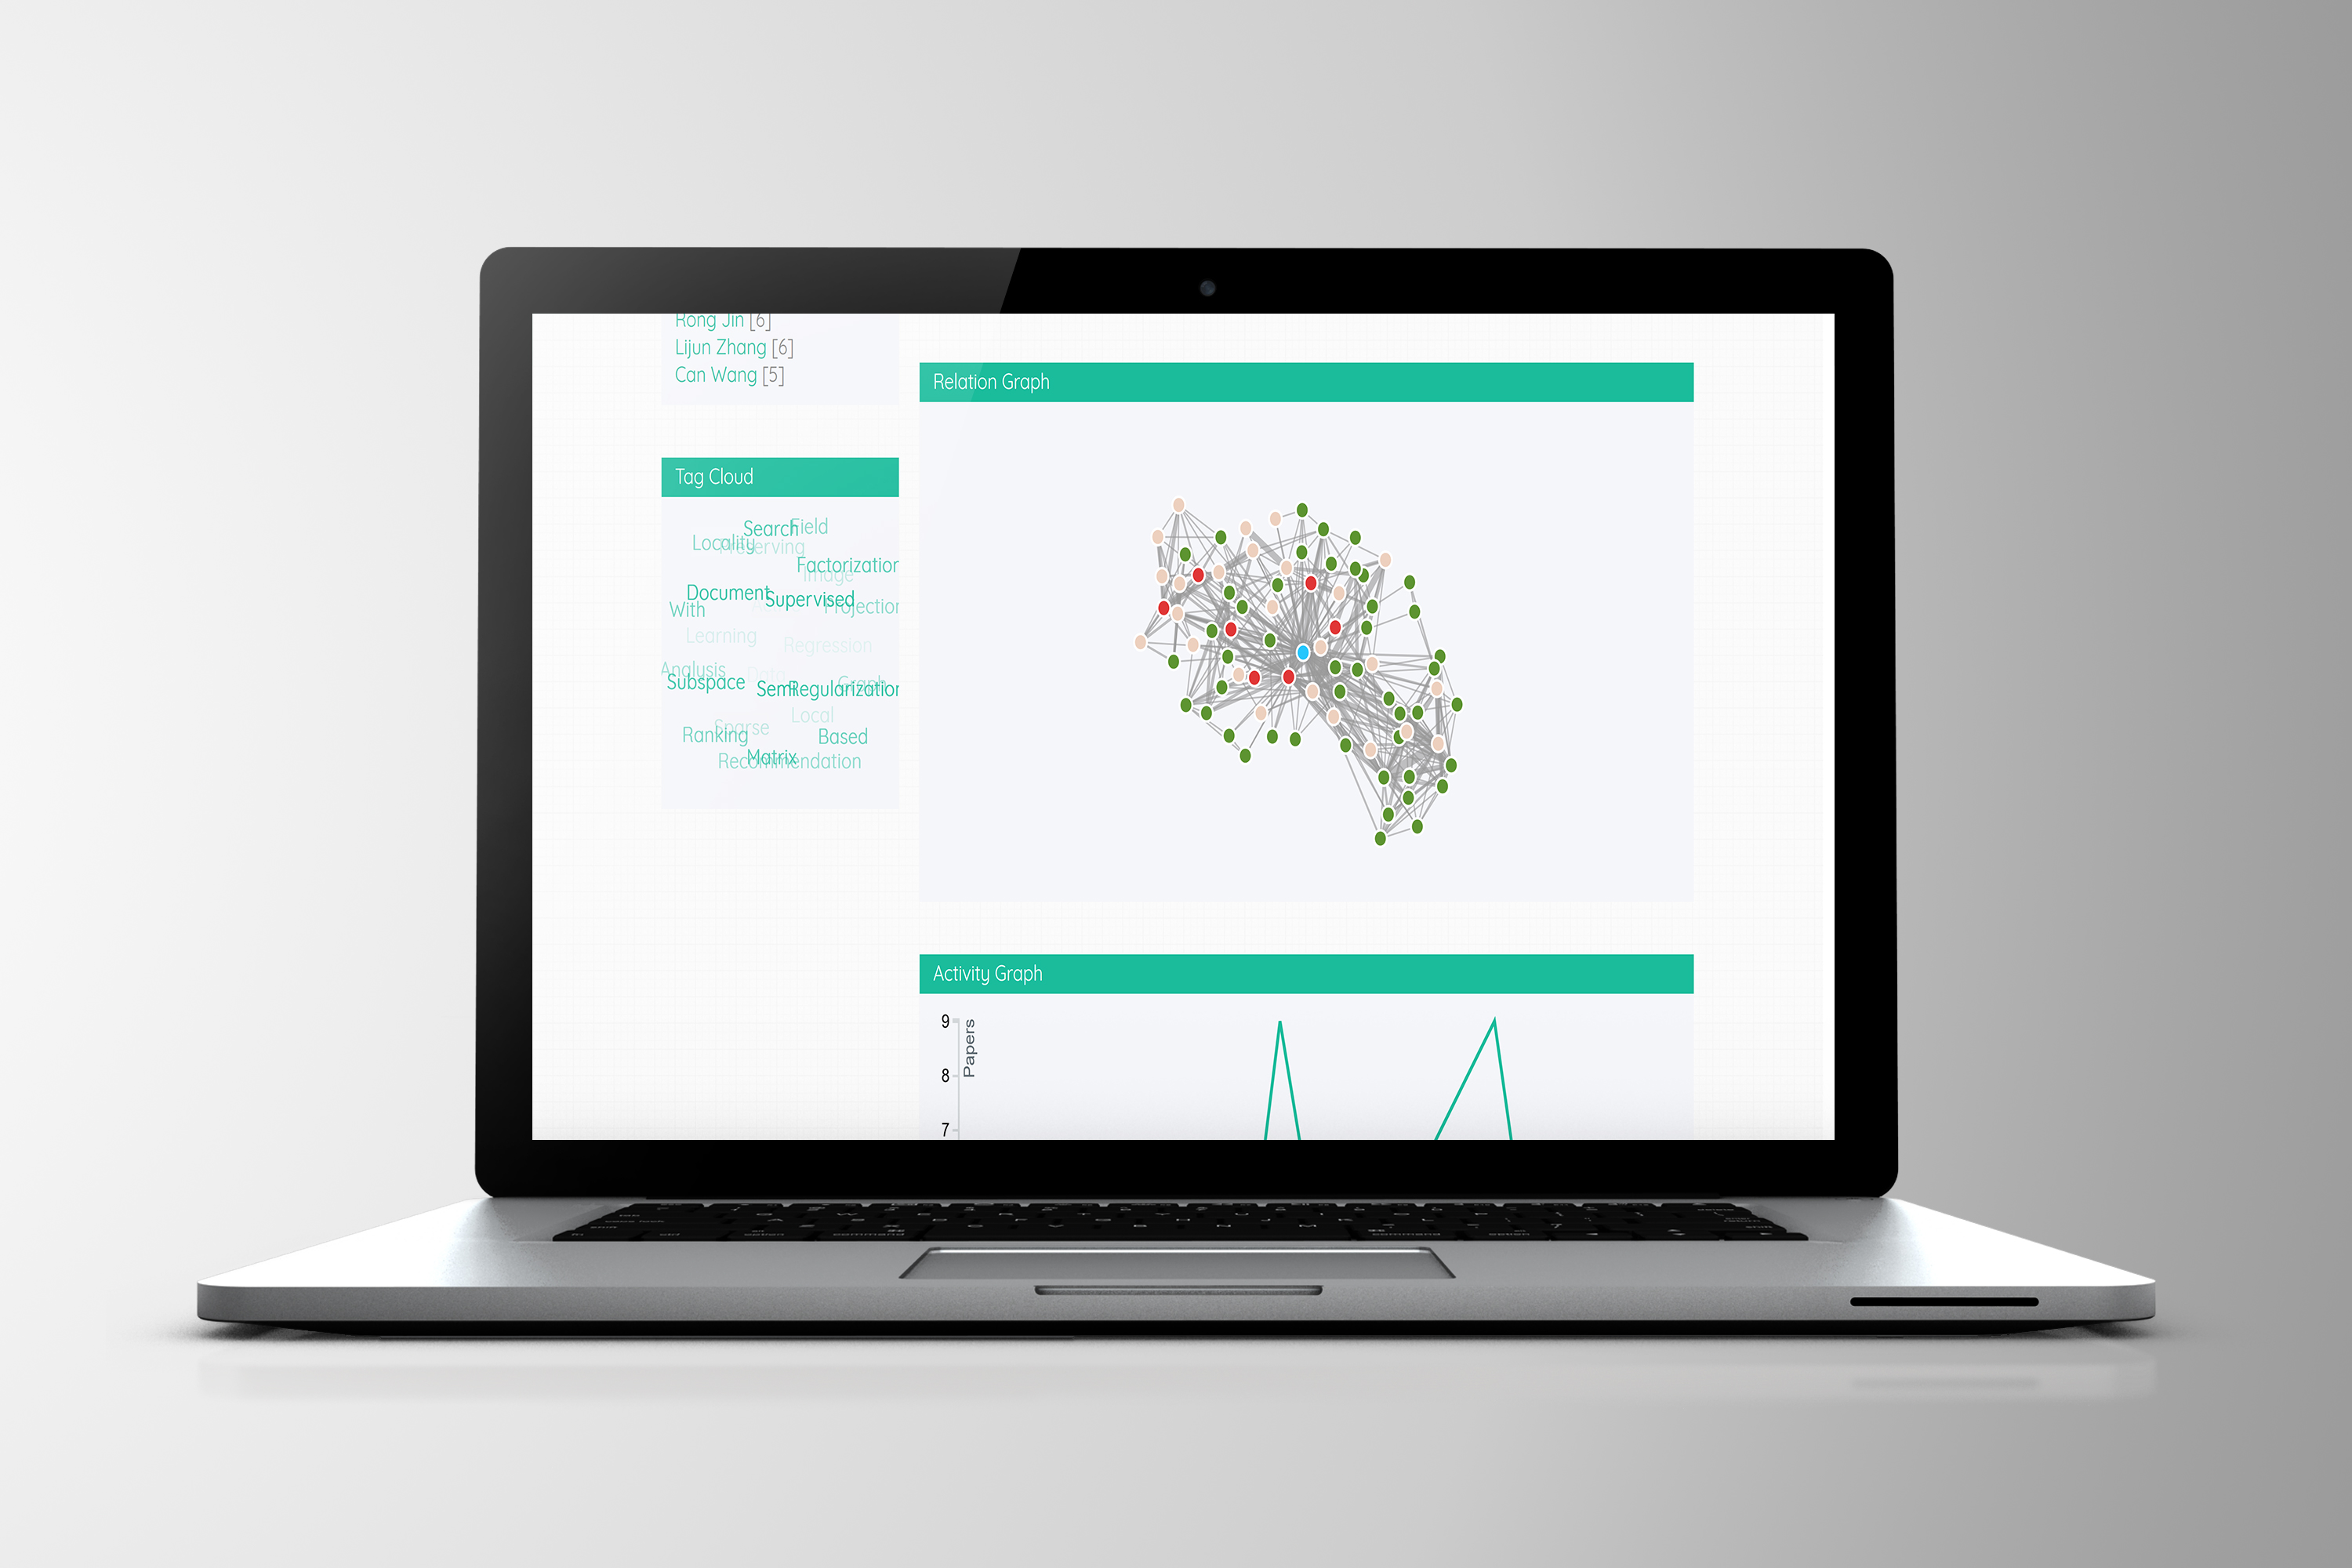
\includegraphics[width=.8\textwidth]{img/img3.jpg}
            \caption{Author}
            \end{figure}
                        \begin{figure}[H]
            \centering
            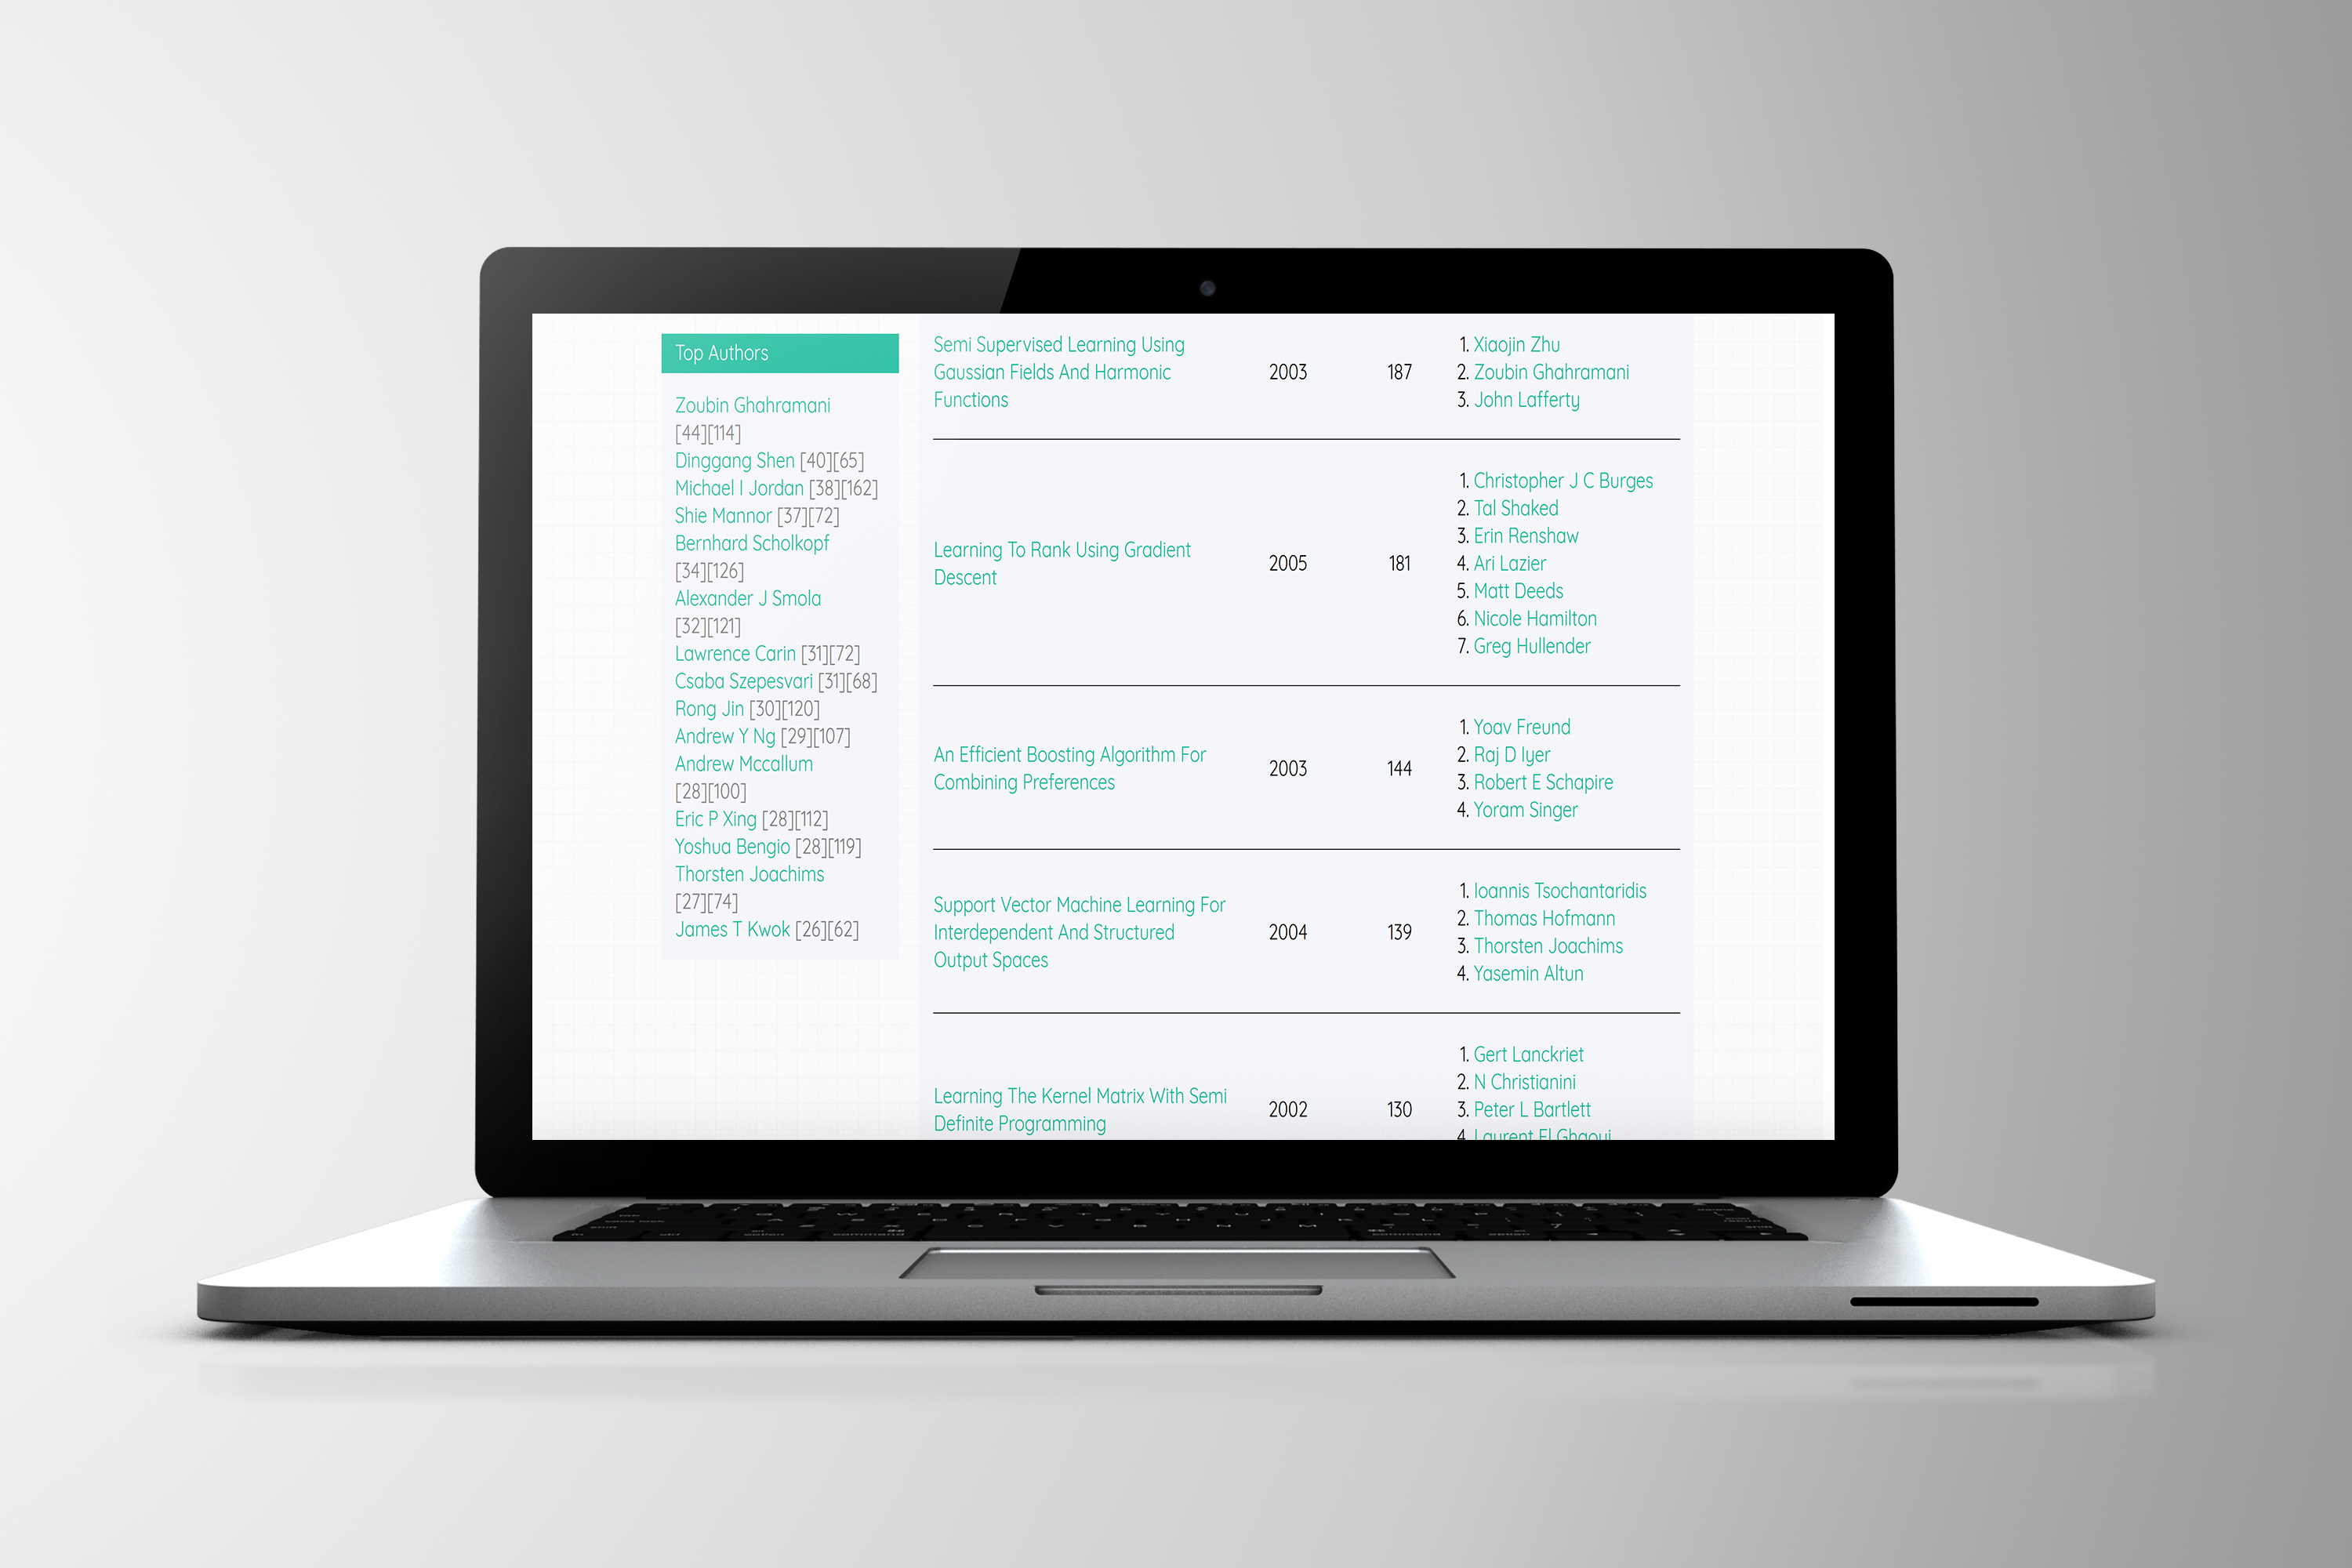
\includegraphics[width=.8\textwidth]{img/img4.jpg}
            \caption{Conference}
            \end{figure}
                        \begin{figure}[H]
            \centering
            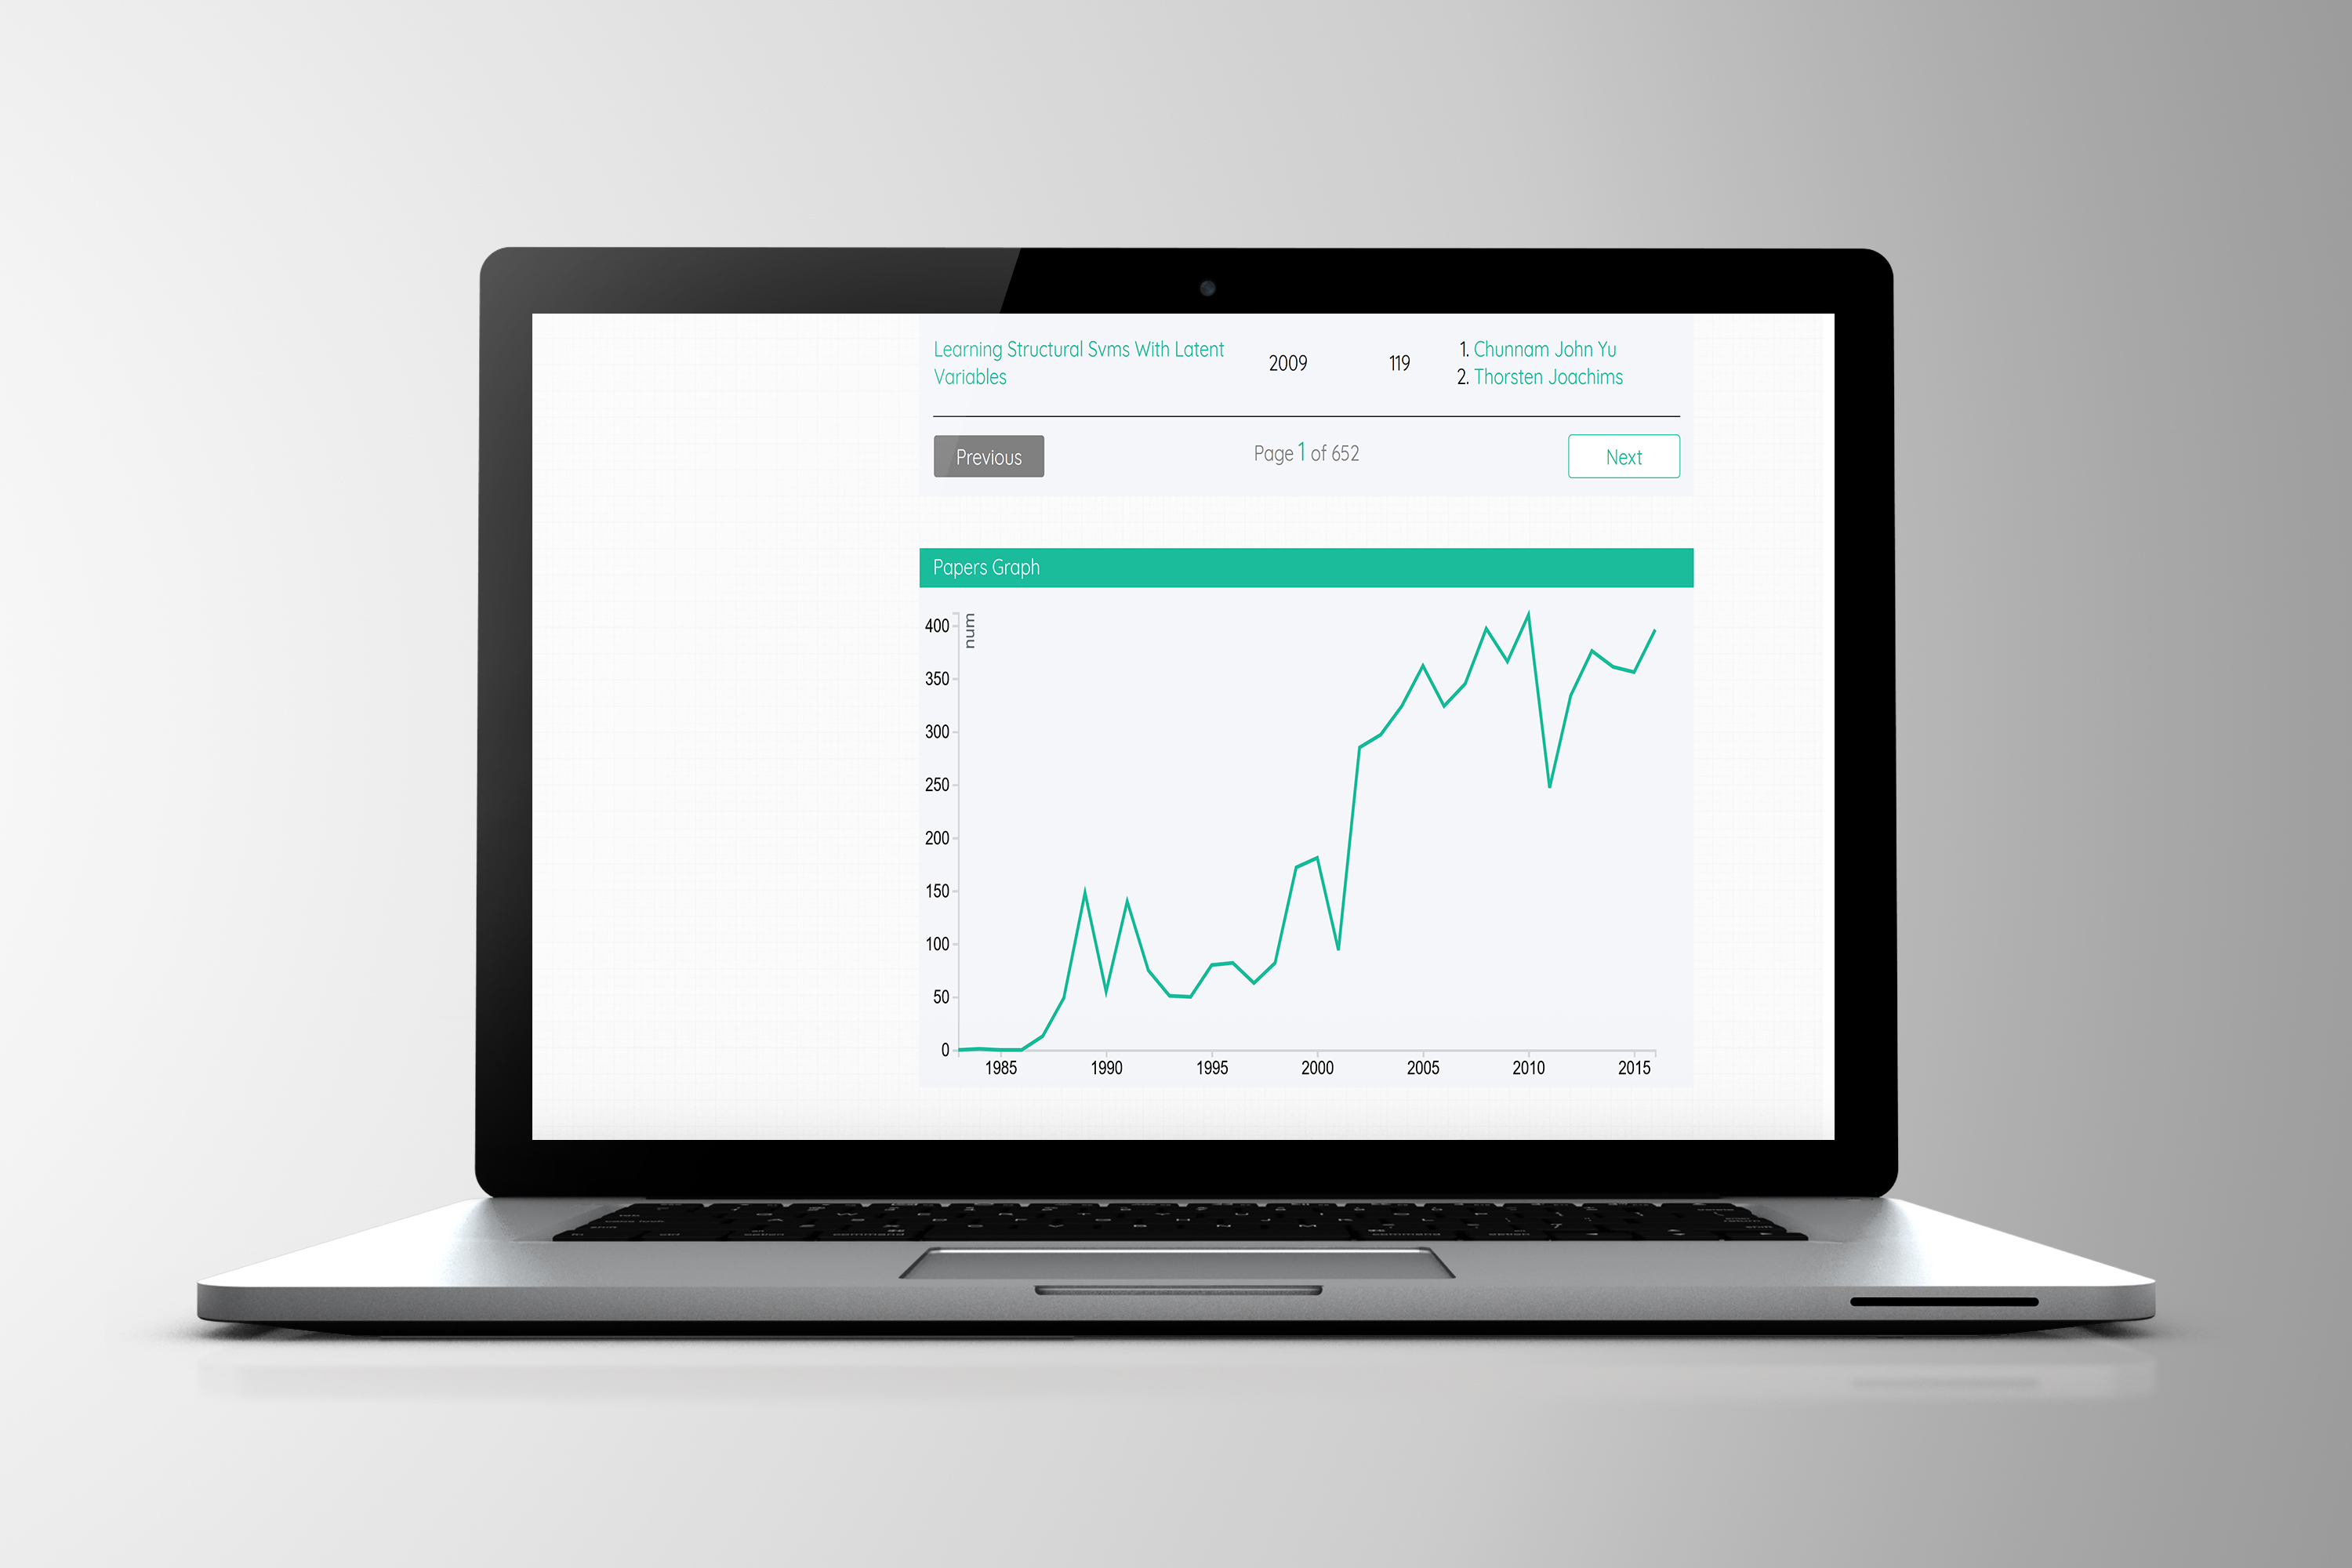
\includegraphics[width=.8\textwidth]{img/img5.jpg}
            \caption{Conference}
            \end{figure}
                        \begin{figure}[H]
            \centering
            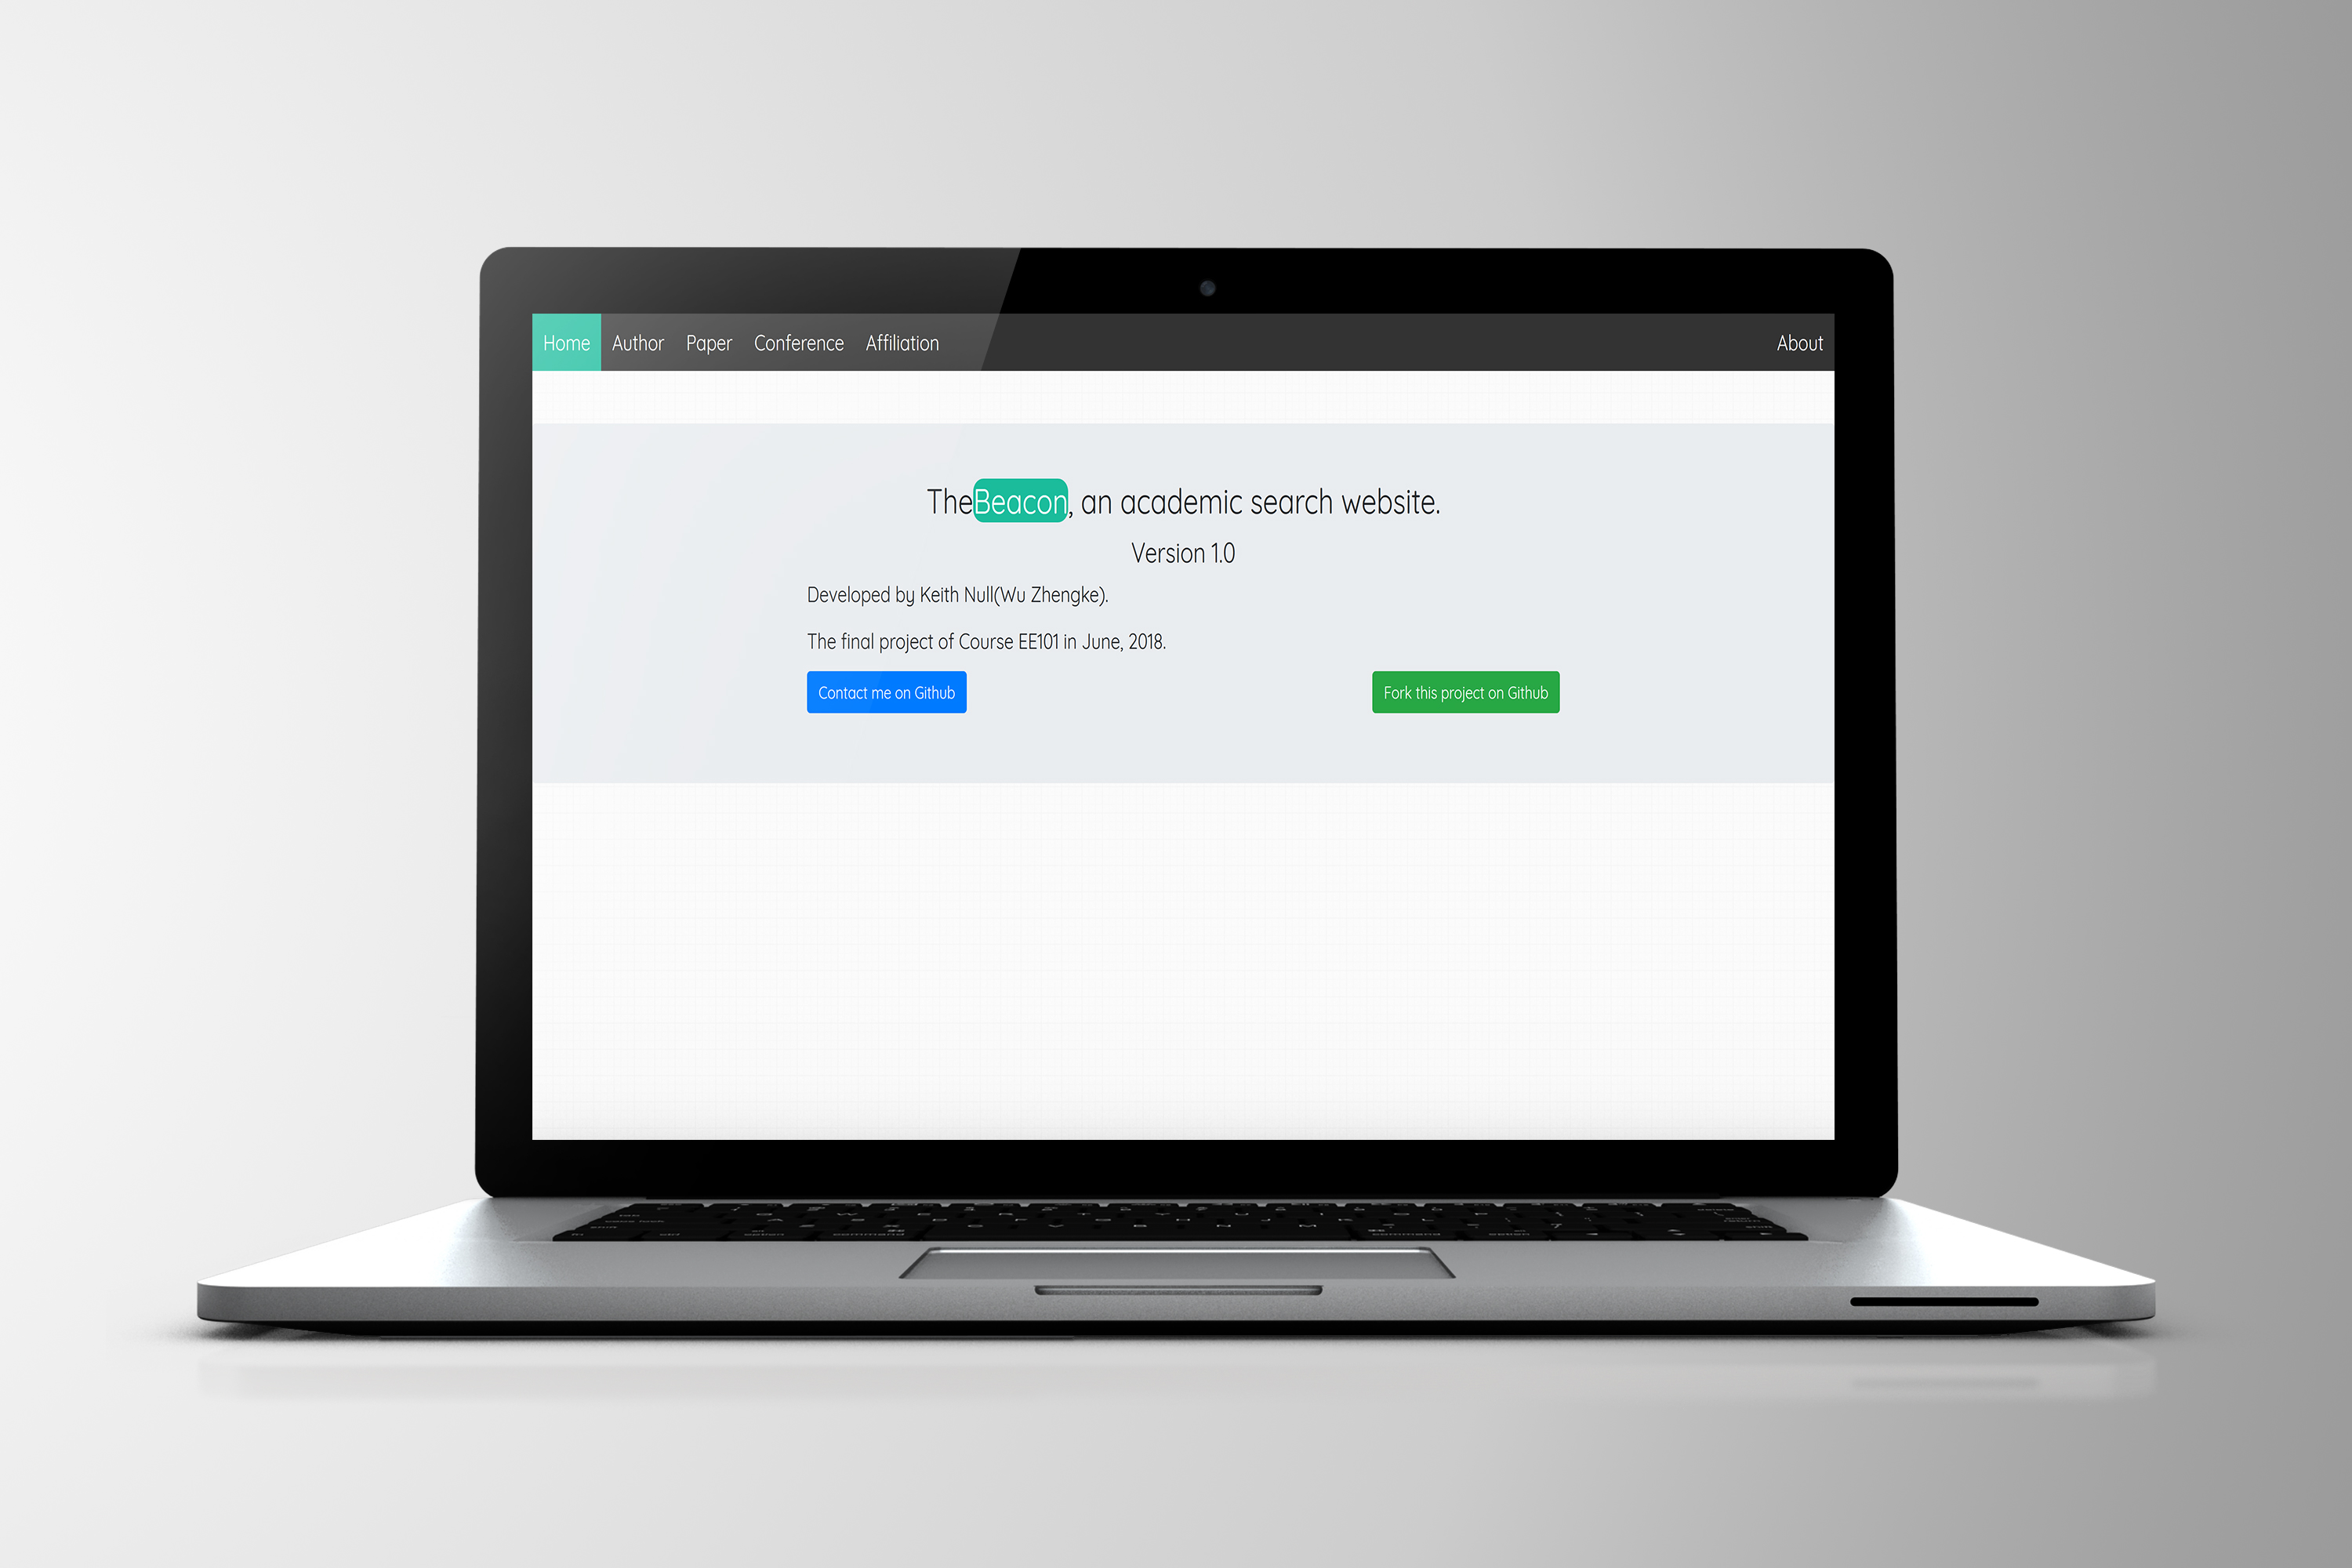
\includegraphics[width=.8\textwidth]{img/img1.jpg}
            \caption{About}
            \end{figure}
    \newpage
    \section{Conclusion and Prospect}
When writing this report, the biggest trouble is that what I have done is something complex but hard to illustrate.
And there're plenty of details that can't be listed here in the report, such as the alignment and offset of 
just a few pixels.

Also, many small features of the website are not illustrated in this report, though I think they are important and
take me much time. (But I have demonstrated them in the presentation.)

Of course, what I have done is far from the state of art, but for me, I feel quite satisfied about it. 

From back-end to front-end, mixing PHP, Python, JavaScript, HTML and CSS, I have learned and practised 
quite a lot. What's more, I have deployed the website on Ali Cloud, during which
I learnd much about Linux and Network...

And as I did all the project by myself instead of in a group, I gain a clear understanding of the 
whole process of buliding a website. It's a unique and memorable experience for me, tiring as it is.

I am not sure whether I will go further to the field of web development in the future. But it's certain
that what I have learned about it now will add more possibility to my future. 

And that's the point of my time and energy devoted to this project.



 
\end{document}
